\documentclass[border=4pt]{standalone}
\usepackage{tikz}
\usepackage{pgfplots}
\pgfplotsset{compat=1.18}
\usetikzlibrary{shapes.geometric,arrows.meta,positioning,calc,fit,decorations.pathreplacing,backgrounds}
\definecolor{boxblue}{RGB}{225,238,252}
\definecolor{boxgreen}{RGB}{225,247,231}
\definecolor{boxorange}{RGB}{253,236,216}
\definecolor{boxgray}{RGB}{237,237,237}
\definecolor{boxred}{RGB}{253,226,226}
\begin{document}
\begin{tikzpicture}[
  box/.style={draw, rectangle, rounded corners, minimum height=0.85cm, minimum width=6.4cm, align=center, font=\small},
  dec/.style={draw, diamond, aspect=3.2, align=center, font=\footnotesize, inner sep=2pt, minimum width=6.4cm},
  arr/.style={-{Latex[length=2.5mm]}, thick}
]
\node[box, fill=boxblue] (i1) at (0,0) {Assumi un valore di tentativo $T_{w,e}$};
\node[box, fill=boxblue] (i2) at (0,-1.15) {Calcola $h_e(T_{w,e}, q'')$ — Cooper/Palen (Cap.\,4)};
\node[box, fill=boxblue] (i3) at (0,-2.3) {Calcola $q'' = h_e\,(T_{w,e}-T_{sat})$};
\node[box, fill=boxblue] (i4) at (0,-3.45) {Risali per conduzione: $T_{w,i} = T_{w,e} + q''\,\dfrac{d_o\ln(d_o/d_i)}{2k_m}$};
\node[box, fill=boxblue] (i5) at (0,-4.6) {Calcola $h_i(T_{w,i})$ incluso eventuale termine radiativo (Cap.\,2, 3)};
\node[box, fill=boxblue] (i6) at (0,-5.75) {Calcola $q''_{gas} = h_i\,(T_{gas}-T_{w,i})$};
\node[dec, fill=boxgray] (dec) at (0,-7.15) {Convergenza\\ raggiunta?};
\node[box, fill=boxblue] (adj) at (-4.6,-7.15) {aggiorna $T_{w,e}$\\[1pt]\footnotesize (secante/bisezione)};
\node[box, fill=boxgreen] (done) at (4.7,-8.5) {$q''$, $T_{w,i}$, $T_{w,e}$ convergenti\\ $\rightarrow U_k$ (Livello 5)};

\draw[arr] (i1) -- (i2);
\draw[arr] (i2) -- (i3);
\draw[arr] (i3) -- (i4);
\draw[arr] (i4) -- (i5);
\draw[arr] (i5) -- (i6);
\draw[arr] (i6) -- (dec);
\draw[arr] (dec) -- node[above,font=\footnotesize]{no} (adj);
\draw[arr] (adj) |- (i1);
\draw[arr] (dec) -- node[right,font=\footnotesize]{sì} (done);
\end{tikzpicture}
\end{document}
